\begin{minipage}[b]{0.6\textwidth}
\begin{Exercise}[label = hamos, difficulty = 2, origin = {USAPhO 2009, Halbfinale}, title = {Oszillierendes Drei-Körper-Problem}]
	Zwei Sterne der Masse $M$ befinden sich im Abstand $D$ voneinander, und sind im Orbit um ihren gemeinsamen Schwerpunkt. \\
	Ein kleiner Körper der Masse $m$ ($m\ll M$) bewegt sich entlang der Achse, die senkrecht auf der Orbitebene steht.\\
	Bestimme das Verhältnis der Orbitperioden der beiden Sterne $T_s$ zu der des kleinen Körpers $T_p$.
\end{Exercise}
\end{minipage}
\begin{minipage}[b]{0.4\textwidth}
	\centering
	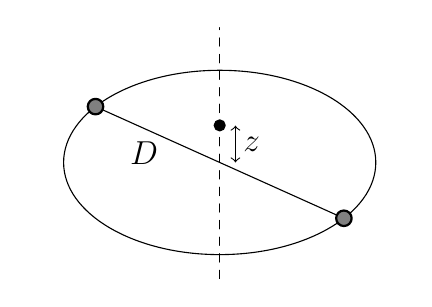
\begin{tikzpicture}[line cap=round,line join=round,x=1.0cm,y=1.0cm, scale = .4]
\clip(-4.096916314848274,-3.6876539866244804) rectangle (7.84614332188144,4.279191433711045);
\draw [rotate around={0.:(2.,0.)}] (2.,0.) ellipse (4.956116965833873cm and 2.9262767092375874cm);
\draw[dashed] (2.,-3.6876539866244804) -- (2.,4.279191433711045);
\draw (-1.943281837397536,1.7726522886577623)-- (5.943281837397535,-1.7726522886577625);
\begin{scriptsize}
\filldraw[fill=gray, draw = black, thick] (-1.943281837397536,1.7726522886577623) circle (7pt);
\draw[fill=gray, draw = black, thick] (5.943281837397535,-1.7726522886577625) circle (7pt);
\draw [fill=black] (2.,1.1770856773113212) circle (5pt);

\draw[<->] (2.5,0) -- (2.5,1.17) node[midway, right] {\large $z$};
\node at (-0.4,0.3) {\large $D$};
\end{scriptsize}
\end{tikzpicture}
\end{minipage}
\begin{Answer}[ref = hamos]
	Der Schwerpunkt des Systems befindet sich bei $r = \frac{D}{2}$. Wir können jetzt die Umlaufzeit durch die korrespondierende Kreisbahn ausrechnen, indem wir dort Gravitations- und Radialkraft gleichsetzen,
	\begin{equation}\label{hamos:ts}
		\frac{m\Gamma}{D^2} = m \left(\frac{2\pi}{T_s}\right)^2 r \Rightarrow T_s = 4\pi\sqrt{ \frac{R^3}{\Gamma}}.
	\end{equation}
	Auf den kleinen Körper wirken jetzt die Gravitationskräfte der beiden Sterne. Zu denen befindet er sich jeweils im Abstand 
	\begin{equation}
		d = \sqrt{r^2+z^2}.
	\end{equation}
	Wenn wir jetzt die wirkenden Kraft ausrechnen, müssen wir beachten, dass sich die Anteile senkrecht zur Bahnachse aufheben, sodass nur noch der entlang der Bahnachse übrig bleibt.
	Dieser ist gegeben durch
	\begin{equation}\label{hamos:fe}
		F =- 2\frac{\Gamma m}{r^2+z^2} \cdot \underbrace{\frac{z}{\sqrt{r^2+z^2}}}_{=\sin \alpha} = 2\Gamma m\cdot \frac{z}{\left(r^2+z^2\right)^{\nicefrac{3}{2}}},
	\end{equation}
	wobei $\alpha$ der Winkel am Stern im rechtwinkligen Dreieck zwischen Orbitmittelpunkt, Stern und dem kleinen Körper ist.\\
	Wir können jetzt den Ausdruck im Nenner als taylorentwickeln, weil wir davon ausgehen können, dass $\frac{z}{r}\ll 1$ gilt. Dann kommen wir
	\begin{equation}
		F \approx - \frac{2\Gamma m}{r^3}z,
	\end{equation}
	was einer hamonischen Schwingung mit Periode 
	\begin{equation}
		T_p =2\pi  \sqrt{\frac{R^3}{\Gamma}}
	\end{equation}
	entspricht. Damit beträgt das gesuchte Verhältnis 
	\begin{equation}
		\boxed{
			\frac{T_p}{T_s} = \frac{1}{2}.
			}
	\end{equation}
\end{Answer}